\documentclass{amsart}

%\documentclass{amsart}
\usepackage[utf8]{inputenc}
\usepackage{amsfonts}
\usepackage{amsmath}
\usepackage{amssymb}
\usepackage{amsthm}
\usepackage{asymptote}
\usepackage{mathtools}
\usepackage{hhline}
\usepackage{graphicx,enumerate}
\usepackage{hyperref}
\usepackage[a4paper, margin=1.2in]{geometry}
%\usepackage{tcolorbox}
\usepackage{tikz-cd}
\usepackage{ytableau}
%\tcbuselibrary{skins,breakable,xparse}
\allowdisplaybreaks
\newcounter{count}
\hypersetup{
	colorlinks=true,
	linkcolor=teal,
	filecolor=magenta,      
	urlcolor=olive,
	citecolor=teal,
	pdfpagemode=FullScreen,
}

%\definecolor{defcolor}{HTML}{478EFF}
%\definecolor{thmcolor}{HTML}{CC0058}
%\definecolor{excolor}{HTML}{F5B400}
%\definecolor{probcolor}{HTML}{DD4803}
%\definecolor{lemcolor}{HTML}{741FEA}
%\definecolor{scarlet}{HTML}{A81111}
%
%\newtheoremstyle{definitionStyle}% Custom style for definitions
%{0.5em}% Space above
%{0.5em}% Space below
%{}% Body font
%{}% Indent amount
%{\bfseries\color{defcolor}}% Theorem head font: bold and red
%{.\\}% Punctuation after theorem head
%{0.5em}% Space after theorem head
%{\thmname{#1}\thmnumber{ #2 (#3)}}% Theorem head spec
%
%\theoremstyle{definitionStyle}
%\newtheorem{df}{Definition}[section]
%
%\newtheoremstyle{theoremStyle}% Custom style for definitions
%{0.5em}% Space above
%{0.5em}% Space below
%{}% Body font
%{}% Indent amount
%{\bfseries\color{thmcolor}}% Theorem head font: bold and red
%{.\\}% Punctuation after theorem head
%{0.5em}% Space after theorem head
%{\thmname{#1}\thmnumber{ #2 (#3)}}% Theorem head spec
%
%\theoremstyle{theoremStyle}
%\newtheorem{thm}{Theorem}[section]
%
%\newtheoremstyle{lemmaStyle}% Custom style for definitions
%{0.5em}% Space above
%{0.5em}% Space below
%{}% Body font
%{}% Indent amount
%{\bfseries\color{lemcolor}}% Theorem head font: bold and red
%{.\\}% Punctuation after theorem head
%{0.5em}% Space after theorem head
%{\thmname{#1}\thmnumber{ #2 (#3)}}% Theorem head spec
%
%\theoremstyle{lemmaStyle}
%\newtheorem{lem}{Lemma}[section]
%\newtheorem{cor}{Corollary}[section]
%
%\newtheoremstyle{exampleStyle}% Custom style for definitions
%{0.5em}% Space above
%{0.5em}% Space below
%{}% Body font
%{}% Indent amount
%{\bfseries\color{excolor}}% Theorem head font: bold and red
%{.\\}% Punctuation after theorem head
%{0.5em}% Space after theorem head
%{\thmname{#1}\thmnumber{ #2 (#3)}}% Theorem head spec
%
%\theoremstyle{exampleStyle}
%\newtheorem{ex}{Example}[section]
%
%\newtheoremstyle{problemStyle}% Custom style for definitions
%{0.5em}% Space above
%{0.5em}% Space below
%{}% Body font
%{}% Indent amount
%{\bfseries\color{probcolor}}% Theorem head font: bold and red
%{.\\}% Punctuation after theorem head
%{0.5em}% Space after theorem head
%{\thmname{#1}\thmnumber{ #2#3}}% Theorem head spec
%
%\theoremstyle{problemStyle}
%\newtheorem{prob}{Problem}[section]

% For Fun
\newcommand{\club}{\color{teal} \clubsuit}
\newcommand{\heart}{\color{red} \heartsuit}
\renewcommand{\star}{\color{scarlet} \bigstar}
\newcommand{\spade}{\color{violet} \spadesuit}

% Symbols
\newcommand{\A}{\mathcal{A}}
\newcommand{\B}{\mathcal{B}}
\newcommand{\C}{\mathbb{C}}
\newcommand{\D}{\mathcal{D}}
\newcommand{\E}{\mathbb{E}}
\newcommand{\F}{\mathbb{F}}
\newcommand{\G}{\mathcal{G}}
% \renewcommand{\H}{\mathcal{H}} Erdos o
\newcommand{\I}{\mathcal{I}}
\newcommand{\J}{\mathcal{J}}
\newcommand{\K}{\mathcal{K}}
% \renewcommand{\L}{\mathcal{L}}
\newcommand{\M}{\mathcal{M}}
\newcommand{\N}{\mathbb{N}}
\renewcommand{\O}{\mathcal{O}}
\renewcommand{\P}{\mathbb{P}}
\newcommand{\Q}{\mathbb{Q}}
\newcommand{\R}{\mathbb{R}}
\renewcommand{\S}{\mathbb{S}}
\newcommand{\T}{\mathbb{T}}
\newcommand{\U}{\mathcal{U}}
\newcommand{\V}{\mathcal{V}}
\newcommand{\W}{\mathcal{W}}
\newcommand{\X}{\mathcal{X}}
\newcommand{\Y}{\mathcal{Y}}
\newcommand{\Z}{\mathbb{Z}}

\renewcommand{\AA}{\mathcal{A}}
\newcommand{\BB}{\mathcal{B}}
\newcommand{\CC}{\mathcal{C}}
\newcommand{\DD}{\mathcal{D}}
\newcommand{\EE}{\mathcal{E}}
\newcommand{\FF}{\mathcal{F}}
\newcommand{\GG}{\mathbb{G}}
\newcommand{\HH}{\mathbb{H}}
\newcommand{\calH}{\mathcal{H}}
\newcommand{\II}{\mathcal{I}}
\newcommand{\JJ}{\mathcal{J}}
\newcommand{\KK}{\mathcal{K}}
\newcommand{\LL}{\mathcal{L}}
\newcommand{\MM}{\mathcal{M}}
\newcommand{\NN}{\mathcal{N}}
\newcommand{\OO}{\mathrm{O}}
\newcommand{\PP}{\mathcal{P}}
\newcommand{\QQ}{\mathcal{Q}}
\newcommand{\RR}{\mathcal{R}}
\renewcommand{\SS}{\mathcal{S}}
\newcommand{\TT}{\mathcal{T}}
\newcommand{\UU}{\mathcal{U}}
\newcommand{\VV}{\mathcal{V}}
\newcommand{\WW}{\mathcal{W}}
\newcommand{\XX}{\mathcal{X}}
\newcommand{\YY}{\mathcal{Y}}
\newcommand{\ZZ}{\mathcal{Z}}
\renewcommand{\d}{\textrm{d}}
% Greek letters
\newcommand{\ep}{\varepsilon}
\newcommand{\ph}{\varphi}
\newcommand{\de}{\delta}
\renewcommand{\a}{\alpha}
\renewcommand{\b}{\beta}
% Fraktur
\newcommand{\mm}{\mathfrak{m}}
\renewcommand{\aa}{\mathfrak{a}}
\newcommand{\bb}{\mathfrak{b}}
\newcommand{\pp}{\mathfrak{p}}
\newcommand{\qq}{\mathfrak{q}}
% Operators
\DeclareMathOperator{\Div}{div}
\DeclareMathOperator{\Gal}{Gal}
\DeclareMathOperator{\vol}{Vol}
\DeclareMathOperator{\Hom}{Hom}
\DeclareMathOperator{\End}{End}
\DeclareMathOperator{\Ext}{Ext}
\DeclareMathOperator{\Tor}{Tor}
\DeclareMathOperator{\tr}{tr}
\DeclareMathOperator{\rk}{rk}
\DeclareMathOperator{\curl}{curl}
\DeclareMathOperator{\mesh}{mesh}
\DeclareMathOperator{\im}{im}
\DeclareMathOperator{\coker}{coker}
\DeclareMathOperator{\width}{width}
\DeclareMathOperator{\diam}{diam}
\DeclareMathOperator{\maps}{Maps}
\DeclareMathOperator{\Frac}{Frac}
\DeclareMathOperator{\Sym}{Sym}
\DeclareMathOperator{\sgn}{sgn}
\DeclareMathOperator{\alt}{Alt}
\DeclareMathOperator{\supp}{supp}
\DeclareMathOperator{\Span}{span}
\DeclareMathOperator{\Var}{Var}
\DeclareMathOperator{\Spec}{Spec}

\newcommand{\nor}{\unlhd}
\DeclareMathOperator{\aut}{Aut}
\DeclareMathOperator{\orb}{Orb}
\DeclareMathOperator{\GL}{GL}
\DeclareMathOperator{\SL}{SL}
\DeclareMathOperator{\SO}{SO}
\DeclareMathOperator{\PGL}{PGL}
\DeclareMathOperator{\PSL}{PSL}
\DeclareMathOperator{\stab}{Stab}
\DeclareMathOperator{\fix}{Fix}
\DeclareMathOperator{\Th}{Th}
\DeclareMathOperator{\Ind}{Ind}
\DeclareMathOperator{\Res}{Res}
\DeclareMathOperator{\Ann}{Ann}
\DeclareMathOperator{\rad}{rad}
\DeclareMathOperator{\len}{len}
\DeclareMathOperator{\ord}{ord}

% \DeclareMathOperator{\arg}{arg}

%% misc
\newcommand{\<}{\langle}
\renewcommand{\>}{\rangle}
\renewcommand{\^}{\wedge}
\renewcommand{\v}{\vee}
\def\Xint#1{\mathchoice
	{\XXint\displaystyle\textstyle{#1}}%
	{\XXint\textstyle\scriptstyle{#1}}%
	{\XXint\scriptstyle\scriptscriptstyle{#1}}%
	{\XXint\scriptscriptstyle\scriptscriptstyle{#1}}%
	\!\int}
\def\XXint#1#2#3{{\setbox0=\hbox{$#1{#2#3}{\int}$ }
		\vcenter{\hbox{$#2#3$ }}\kern-.6\wd0}}
\def\ddashint{\Xint=}
\def\dashint{\Xint-}
%% arrows
\newcommand{\xhra}{\xhookrightarrow}
\newcommand{\xra}{\xrightarrow}
\newcommand{\ra}{\rightarrow}
\newcommand{\rra}{\rightrightarrows}
\newcommand{\lra}{\longrightarrow}
\newcommand{\Ra}{\Rightarrow}
\newcommand{\lRa}{\Longrightarrow}
\newcommand{\lrsa}{\leftrightsquiqarrow}
\newcommand{\ba}{\leftrightarrow}
%% lists
\newcommand{\be}{\begin{enumerate}[(i)]}
	\newcommand{\ee}{\end{enumerate}}
%% integration stuff
\newcommand{\calR}{\mathcal{R}}
\newcommand{\rint}{\calR\!\int}
\newcommand{\calL}{\mathcal{L}}
\newcommand{\lowerint}{\mbox{\b{$\int$}}}
\newcommand{\upperint}{{\textstyle\bar{\int}}}
%% end of proof
\def\endproof{{\hfill $\Box$}}
%% matrix shorthand

\title{Math 317 HW 3}
\author{Jalen Chrysos}

\begin{document}
	\maketitle

\textbf{Problem 1 (Hatcher 1.2:9)}: In the surface $M_g$ of genus $g$, let $C$ be a circle that separates $M_g$ into two compact surfaces $M_h'$ and $M_k'$ obtained from the closed surfaces $M_h$ and $M_k$ by deleting an open disk from each. Show that $M_h'$ does not retract onto $C$, and hence $M_g$ does not retract onto $C$. But show that $M_g$ does retract onto the non-separating circle $C'$ in the figure.

\begin{center}
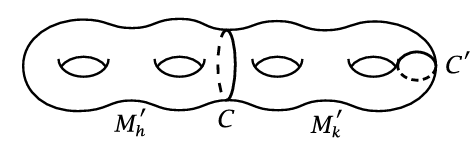
\includegraphics[height=3cm]{"C:/Users/jzchr/MathDocuments/Class Work/Topology/Homework/317HW3/Fig_1.9_Hatcher.png"}
\end{center}

\newpage
\textbf{Problem 2 (Hatcher 1.2:11)}: The mapping torus $T_f$ of a map $f:X\to X$ is the quotient of $X\times I$ obtained by identifying each point $(x,0)$ with $(f(x),1)$. In the case $X=S^1\vee S^1$ with $f$ preserving basepoints, compute a presentation for $\pi_1(T_f)$ in terms of the induced map $f_*:\pi_1(X)\to\pi_1(X)$. Do the same when $X=S^1\times S^1$.

\newpage
\textbf{Problem 3 (Hatcher 1.2:14)}: Consider the quotient space $X$ of a cube $I^3$ obtained by identifying each square face with the opposite square face via a clockwise quarter-rotation and translation by one unit. Show that $X$ is a cell complex with two $0$-cells, four $1$-cells, three $2$-cells, and one $3$-cell. Using this structure, show that $\pi_1(X)$ is the quaternion group.
\begin{proof}
	
\end{proof}

\newpage 
\textbf{Problem 4 (Hatcher 1.2:16)}: Show that the fundamental group of the surface of infinite genus is free on an infinite number of generators.

\newpage
\textbf{Problem 5 (Hatcher 1.2:22)}: In this exercise, we describe an algorithm for computing the \textit{Wirtinger presentation} of the fundamental group of the complement of a knot in $\R^3$. We begin with the knot lying almost flat on a table $T$ so that $K$ consists of finitely-many disjoint arcs $\a_i$ contained within $T$ and finitely-many $\b_{\ell}$ which leave $T$ to cross over another part of $K$. We build a 2-dimensional complex $X$ that is a deformation retract of $\R^3-K$ in the following steps:\\

For each $\a_i$, let $R_i$ be a curved rectangle so that its long edges are on $T$ and it has $\a_i$ underneath it, and let and $\b_{\ell}$ crossing over $\a_i$ lie along the curve of $R_i$. For each $\b_{\ell}$, let $S_{\ell}$ be the square-shaped piece which covers the crossing. Let $X$ be the union of $T$, $R_i$, and $S_{\ell}$ for all $i,\ell$. Lift $K$ off the table slightly so that it does not intersect $X$. Then we can retract $R^3-K$ to $X$.\\

\begin{enumerate}[(a)]
	\item Assuming that this retraction is possible, show that $\pi_1(\R^3-K)$ has a presentation with one generator $x_i$ for each $R_i$ and one relation $x_ix_jx_i^{-1}=x_k$ whenever $\a_j,\a_k$ are two pieces which cross over $\a_i$ via some $\b_{\ell}$.
	\item Use this presentation to show that the Abelianization of $\pi_1(\R^3-K)$ is $\Z$.
\end{enumerate}

\newpage
\textbf{Problem 6 (Hatcher 1.B:5)}: Consider the graph of groups $\Gamma$ having one vertex $\Z$ and one edge $n\mapsto 2n$. Show that $\pi_1(K\Gamma)$ has presentation $\<a,b|bab^{-1}a^{-2}\>$ and describe the universal cover of $K\Gamma$ explicitly as a product $T\times \R$ with $T$ a tree.

\newpage
\textbf{Problem 7 (Hatcher 2.1:5)}: Compute the simplicial homology groups of the Klein bottle using the $\Delta$-complex structure.

\newpage
\textbf{Problem 8 (Hatcher 2.1:8)}: Construct a 3-dimensional $\Delta$-complex $X$ from $n$ tetrahedra $T_1,\dots,T_n$, with all sharing a common edge and each sharing a face with its two neighbors. Show that the simplicial homology groups of $X$ in dimensions 0,1,2,3 are $\Z,\Z_n,0,\Z$ respectively.

\newpage 
\textbf{Problem 9 (Hatcher 2.1:11)}: Show that if $X$ is a retract of $X$ then the map $H_n(A)\to H_n(X)$ induced by the inclusion $A\subset X$ is injective.

\end{document}